\chapter{Variable Range Hopping}		% chapter 1
\label{theorychap}

\section{History}
In 1937, Nevill Mott and Rudolf Peierls explained why some materials which should have been conductors, acted as insulators. This was due to electron-electron interactions, which is not taken into account in band theory ~\cite{mott72}. From there, Miller and Abrahams proposed a network resistor model which Efros and Schklovskii built on ~\cite{efros75}. Because of the dynamic complexity of even a small system (a 10 by 10 system can have $2^{100}$ configurations) simulations are a large part of modern electron hopping studies ~\cite{kirkengen09}. The theory has gotten more consise over time. For the sake of simulation, much of it can be compressed into equation~\ref{probability}.

Transport through a quantum dot which is weakly coupled to two conducting leads is dominated by the electron-electron interaction ~\cite{Glazman05}. When the thermal energy is not enough to overcome the charging energy of the dot, coulomb blockade takes over and resistance is increased. At low enough temperatures, the Kondo effect takes over. That is when the magnetic field of the electrons starts to matter energy-wise. At that point, electrons start to prefer states where they are anti-parallel.

Kinetic monte carlo methods are useful when simulating condensed matter systems which include time evolution. There are two types, rejection and rejection-free, the difference being whether or not an event has a chance of failing all-together. If a kinetic Monte Carlo method is also subject to detailed balance, then it simulates a system at thermodynamic equilibrium~\cite{Young66}. A kinetic monte carlo method is useful for modeling variable range hopping. The temperature dependence of conductivity can be tested using a kinetic Monte Carlo algorithm. If one assumes that single-particle excitations are responsible for variable range hopping, then one ends up with the Efros-Shklovskii law:
\begin{eqnarray}
\sigma_c \approx (\gamma e^2 / T) \exp(-(T_0/T)^{1/2}),
\label{ESlaw }
\end{eqnarray}
Where $\sigma_c$ is the conductivity, $\gamma$ is the frequency, $T$ is the temperature, and $T_M = \beta_M (g_0 a^2)^{-1}$ where $a$ is the localization length of the electron, $g_0$ is the density of states at the Fermi level, and $\beta_M$ is a numerical coefficient.~\cite{Tsigankov02} show that single electron jumps are sufficient to describe the system. This is important since otherwise we would have to simulate multi-electron jumps which would scale the difficulty of simulation by an order of magnitude. The problem of studying this situation increases with decreasing temperature as electrons are able to jump farther. 

The Coulomb glass system was found to be robust enough to relax within simulateable times. ~\cite{Kirkengen09} Found that the relaxation time is slightly slower than exponential. Energy correlations at equilibrium however were found to be exponential:
\begin{eqnarray}
C(\tau) = e^{-(\tau / \tau_0)^\gamma},
\label{correlations}
\end{eqnarray}
where $\gamma$ is proportional to temperature at low temperatures, and $\tau , \tau_0$ are time dependent. Only at low temperatures below $T_{min} \approx 0.02$ does the system take too long to equilibrate. The behavior is similar to that of a random walk on a fractal configuration space. 

The Coulomb glass is applicable to nanoscale nanular lattices, and much research has been conducted on them. Abeles et. al. did some of the original work on nano-granules. They achieved this by co-sputtering metals and insulators. They attributed conduction due to electron percolation and tunneling. They also define a charging energy required to tunnel as $E_j = e^2/2C$ where $C$ is an effective junction capacity. Another interesting phenomenon that they observed was that of the electric field breakdown. That is, if the voltage drop between particles became comparable to the height of the tunneling barrier, then electrons could go straight into the conduction band of the insulator. 

In ~\cite{Vinokur08} The 2D lattice of Coulomb glasses with site disorder was studied. When the effect of site disorder was on the same scale as the Coulomb energy, the distribution of local minima becomes exponential. At low disorder, the density of states becomes crystal-like. They also found that in order to fully relax a system, multiple-electron jumps must be taken into account. 

Eventually, arrays of nano-scale metallic particles were able to be embeded in insulating matrices. These metallic particles act like artificial atoms with programable electronic properties. These can be formed such that they are insulators, conductors, semiconductors, or even superconductors. ~\cite{Beloborodov07}  Were able to show that there was logarithmic temperature dependence of the conductivity. This system also appears to show negative magnetoresistance under certain parameters. 

By tuning the ability of electrons to travel, one can also start to change the Seebeck coefficient of the material. ~\cite{Glatz09} derive the thermopower and thermoelectric coefficient of nanogranular materials. They find the thermoelectric coefficient to be:
\begin{eqnarray}
\eta = \eta^{(0)} (1 - \frac{1} {4 g_T d} ln \frac{g_T E_c} {T} ),
\label{thermoelectric}
\end{eqnarray}
where $\eta^{(0)} = -(\pi^2 / 3) e g_T a^{2-d} (T/ \epsilon_F)$, $a$ is the size of a grain, $d$ is the dimensionality of the system, $\epsilon_F$ is the Fermi energy, and $E_c = e^2 /a$ is the charging energy. 


\section{Monte Carlo methods}
Monte Carlo methods are a randomized way to use the law of large numbers to find answers to mathematical and physical problems. For example, In oil and space exploration, Monte Carlo methods are a better predictor of cost overruns than human intuition~\cite{Hubbard09}. While there is no consensus on the exact definition of a Monte Carlo method, One can get a feel for it by looking at simple examples. Some good examples are the estimation of $\pi$ and the Metropolis method. 

\subsection{Estimating $\pi$}
Estimating $\pi$ has been a challenge for mathematicians since ancient Egyptian times. One possible method is by trying a Monte Carlo strategy. For simplification, one usually just takes a fourth of a circle inscribed in a square (see fig.~\ref{piSquare}). One then picks random numbers between 0 and 1 for x and y. Success is then defined as ~\cite{Kalos08}:
\begin{eqnarray}
\sqrt{x^2 + y^2} < 1 .
\label{piSuccess}
\end{eqnarray}
In a way, all we are doing is integration. If one counts the number of successes and divides by the number of total trials, it will equal to the ratio of the area of the quarter circle and the square of length 1, which can then be solved for $\pi$. Integration of this sort can be used to approximate the area under any integrable curve, and in the case of the "pathological equation" some non-integrable ones as well~\cite{Newmann99}. 

\subsection{Metropolis method}
The Metropolis algorithm is a way to draw samples from a probability distribution iteratively. Because each distribution is only affected by the previous distribution, this can be considered a Markov chain. A Markov chain is simply a sequence of random variables which a system moves through with serial dependence. In its simplest sense, we have
\begin{eqnarray}
\overrightarrow X_{t+1} = \overrightarrow{ \overrightarrow Q} \overrightarrow X_{t} ,
\label{Markov}
\end{eqnarray}
where $\overrightarrow X_t$ is the state of the system at step $t$, and $\overrightarrow{\overrightarrow Q}$ is the probability matrix. Under certain circumstances, the probability matrix can be applied multiple times, eventually causing the state to approximate an equilibrium~\cite{Everitt02}. The Metropolis method can be used for many systems, but we will focus on the Ising problem as it is similar to our problem.

\subsection{Ising problem}
The Ising method is a way to solve the problem of dipole moments on a large array of atoms. While the Hamiltonian can be fairly simple ~\ref{Ising}, its properties such as its specific heat or hysteresis can be relatively complex.   
The Hamiltonian is 
\begin{eqnarray}
H(\sigma) = - \Sigma J_{ij} \sigma_i \sigma_j - \mu \Sigma h_j \sigma_j , 
\label{Ising}
\end{eqnarray}
where $\sigma_i$ is the spin, $J_{ij}$ is the interaction strength between neighbors, $\mu$ is the magnetic moment, and $h_j$ is an external magnetic field. Then the configuration probability is:
\begin{eqnarray}
P(\sigma) = \frac {e^{-\beta H(\sigma) }} {Z_\beta },
\label{configurationProbability}
\end{eqnarray}
where $\beta = (k_B T)^{-1}$, and the renormalization constant $Z_\beta = \Sigma e^{-\beta H(\sigma)}$. From here we have a 3 step process to simulate the system. First, we must choose an arbitrary configuration to be our starting point. Next, we pick an adjacent configuration in configuration space (i.e. a configuration that we can get to by just changing one value). If going there is energy favorable, then the change is made. Otherwise, the change is made accoring to the probability ~\ref{configurationProbability}. As the system is evolved, variables such as magnetic field and temperature can be changed, which can lead to properties such as specific heat and hysteresis. 

\section{Jump Probability}

In order to calculate were the electron will jump, we must first find the probability of each jump site. Our main equation involved is as follows:
\begin{eqnarray}
P_{ij} = \exp (-2\alpha R_{ij} -  E_{ij}/kT)
\label{probability}
\end{eqnarray}

where $k$ is the Boltzmann constant, $R_{ij}$ is the distance between cells, $E_{ij}$ is the energy change of the system if a particle were to move from i to j, and T is the temperature of the system.$\alpha = \sqrt{2mH/\hbar}$ where $m$ is the effective mass at the bottom of the conduction band and $H$ is the mean energy of the conduction band. $\alpha$ is set up to be around the same scale as the inter-grain distance. $E_{ij}$ has various inputs which vary in energy scale~\cite{Mott68}.
\begin{eqnarray}
E_{ij} =  \triangle U_{ij} e^2/a\kappa_1  + e f_i \triangle V_{ij} + f_i  \triangle \mu_{ij} + f_i (eV) \triangle x_{ij} 
\label{deltaE}
\end{eqnarray}
where $i$ refers to the starting site index and $j$ refers to the target site index,  $f$ is the occupation of a site, $a$ is the size of the granule, $\kappa_1$ is the intra-granule dielectric constant, $\mu$ is the substrate potential, $V_{ij} = \sum_{n=1}^{N} e^2/\kappa_2 r_{n}$ is the local potential from the rest of the particles, $\kappa_2$ is the inter-granule dielectric constant, $\triangle x$ is the component of r in the direction of eV , and $eV$ is an externally applied voltage. $\triangle U_{ij}$ is -1 if electrons stacked, 1 if electrons de-stacked, and 0 otherwise. The first two components of equation ~\ref{deltaE} together constitute the electrostatic component of this system. The most powerful is the Coulomb blockade. This introduces a large penalty into the probability of an electron occupying the same site as another electron. If the site at which an electron can travel to is empty, the chances of transport are higher than if the site is filled ~\cite{glazman05}. There is also a contribution from the substrate. There is an inherent randomness in the potential at different lattice sites and that is where this comes in. This energy landscape somewhat randomizes starting energies and can fill in as electron donor. There is a general electric potential which will try to get the electrons to space out evenly in the substrate (periodic boundary conditions). Finally there is a current portion which if a voltage bias is applied on the left and right sides of the system, then the probability of electrons hopping with that bias is increased ~\cite{aharony92}. The exponential term is artificially limited below 0 to keep the electron hop ranges realistic. Analytically, equation~\ref{probability} can be maximized to find the most common jump distance (take the derivative with respect to r and set equal to 0). In our case, there are 2 problems with this approach. First, we are more interested in the average jump distance which need not be the maximum. Second, The analytical approach assumes a continuous system, where in reality it is a discrete number of interacting points. There are a few nuances in the theory that need to be adressed.
\subsection{Mott vs. Effros-Schklovskii}
While the approach to describe physical systems by Mott vs Effros-Schklovskii (ES) theory are similar, there are a few key differences in the details. First, The localization parameters are different due to differences in the density of states. The localization is temperature dependent in the ES system. This is because ES considered the situation where if an electron tries to tunnel, It must leave an electron hole behind. This enhanced requirement for the energy means that at low temperatures, the density of states at the Fermi level vanishes ~\cite{joung}. The resistivity for the Mott system ends up being related to the temperature as

\begin{eqnarray}
\ln(\rho) \approx (T_o / T)^{1/4} ,
\label{fourth}
\end{eqnarray}
where $\rho$ is the resistivity and $T$ is the temperature. Meanwhile, in the ES system we have
\begin{eqnarray}
\ln(\rho) \approx (T_o / T)^{1/2}.
\label{half}
\end{eqnarray}
The Mott resistance comes from $\delta E = \alpha_1 / g r_{ij}^3 $, where $\alpha_i$ are prefactors of order unity. The ES resistance comes from the usual Coulomb blockade term $\delta E = \alpha_2 e^2 / \kappa r_{ij}$ ~\cite{aharony92}. The Differences can be summarized in a single plot ~\ref{MvsES} ~\cite{Liu10}.

\begin{figure}[htbp]
\begin{center}
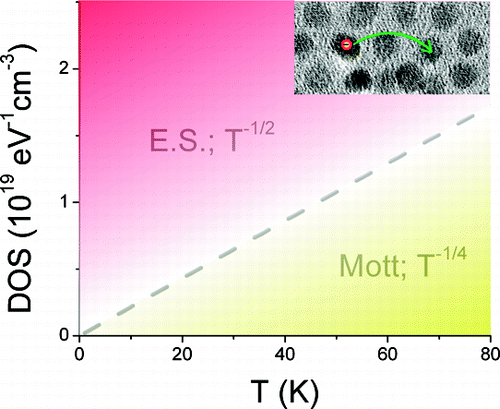
\includegraphics[scale=.50]{MottvsES.png}
\caption{Density of states vs Temperature. This plot describes the interface between ES and Mott transmission of electrons. (Graph courtesy of Heng Liu)}
\label{MvsES}
\end{center}
\end{figure}

\subsection{Coulomb Glass vs Artificial Nanosolids}
Coulomb glasses are the original substrate on which the ES model of electron conduction was based. The "glass" in coulomb glass refers to a phase in which electron-electron interactions impair conduction and dynamics become slow, like the flow of a glass~\cite{ortuno04}. Artificial nanosolids are arrays of granules which have a higher intra-granule conduction than a inter-granule conduction. The differences begin at the density of states. In artificial nanosolids, the density of states can be more creative. By changing the size of the granule, and the material it is made out of (metal, insulator, superconductor) the amount of available electron slots per site (and the energy of each slot) can be chosen. There are two energy scales for each grain. $\delta$ is the mean level spacing. $E_c$, the energy required to pack on one more electron onto a site is on the order of 3000 Kelvin ~\cite{glatz08} .The distances are also different. For coulomb glasses, the distances are basically the inter-atomic distances. There we are basically talking about electron jumps between atoms on a crystal lattice. As the name suggests, in artificial nanosolids the distances are arbitrary. For typical artificial nanosolid applications, we are in the nanometer to tens of nanometers range~\cite{beloborodov05}. While the general electric potential plays a role in both systems, It plays a bigger role in the coulomb glass since the scales are smaller and the electric potential scales as $1/r$.

\subsection{Inelastic vs. Elastic tunneling}
As well as blocking each other, electrons also can impart energy onto each other which may result in an electron being dislodged. This is referred to as inelastic co-tunneling. If instead the electron tunnels or otherwise travels without dislodging, it is referred to as elastic co-tunneling (see fig. ~\ref{inelasticvselastic}). For low to medium temperatures, the main tunneling mechanism will be elastic. At higher temperatures, we expect a transition to in-elastic tunneling~\cite{Glazman05}.

\begin{figure}[htbp]
\begin{center}
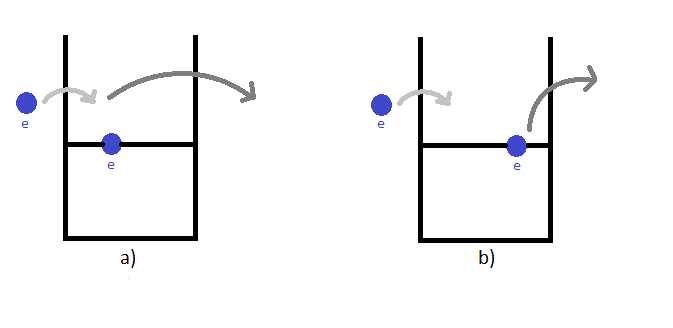
\includegraphics[scale=.50]{inelasticvselastic.png}
\caption{a) elastic transmission of electrons. b) inelastic transmission of electrons.}
\label{inelasticvselastic}
\end{center}
\end{figure}

\subsection{Temperature}

Temperature-dependent phase transitions are scattered throughout the spectrum and so it is important to specify at which temperatures we are working with. At temperatures lower than the Neel temperature, We encounter the first transition called "Mott-Heisenberg". At these low temperatures, the magnetic fields of the electrons have a chance to couple into anti-ferromagnetic pairs. Also, During tunneling events, electrons will avoid atoms which are occupied with other electrons of similar spins as sharing an atom would require an increase in energy compared to one of opposite spin ~\cite{Gebhard03}. At medium temperatures, we have a transition between elastic and inelastic. In order for an electron to land on an occupied site it must have enough energy to overcome the Coulomb blockade. This is only possible if it was given enough kinetic energy from a phonon (sufficient thermal energy). As the temperature is increased, electrons can begin stacking. Once an electron stacks onto another electron, Coulomb repulsion guarantees that either electron will quickly move on~\cite{Glazman05}. At much higher temperatures, the system starts to have enough free thermal energy to exceed the coulomb blockade energy. That is, the energy required to stack 2 electrons in the same quantum dot. This yields a crossover temperature which was discussed during our comparison of ES vs Mott systems ~\cite{aharony92}. Depending on the density of states, there will eventually be higher energy states on which to pack on electrons. For our purposes, we will stay in between these two systems. Our temperatures will be high enough that magnetic moments can be ignored, yet low enough that the maximum number of electrons allowed on the same quantum dot will be two.

\subsection{Density of States}
There are many methods of characterizing the energy of an electron. One of these is the density of states. This is a histogram of the energies that electrons can be in. For example in ~\ref{moundDoS}, there are many electrons at a relatively low energy and the number of electrons with higher energies decreases with energy. In ~\ref{crystalDoS} there is only one energy option for electrons. We see two peaks because the holes act as particles in that the system requires energy to move those as well. The value on the x axis is the energy required to fill or empty each hole or particle respectively. By knowing the shape of the density of states, one can discern important intricacies of a system. These can include the energy scales, the relaxedness, and the bandgap of a system. The typical kinetic energy of an electron in a fermi glass is $E = E_o + \frac{(\hbar k)^2} {2m}$. If one follows through the math, the dispersion relation ends up as $D_n(E) = \frac {nc_n} {p c^{n/p}_k} (E- E_o)^{n/p-1}$ ~\cite{Kittel96}. If the particle distribution is symmetric (same amount of electrons as holes) then the density of states will be symmetric, as long as the system is relaxed.

\begin{figure}[htbp]
\begin{center}
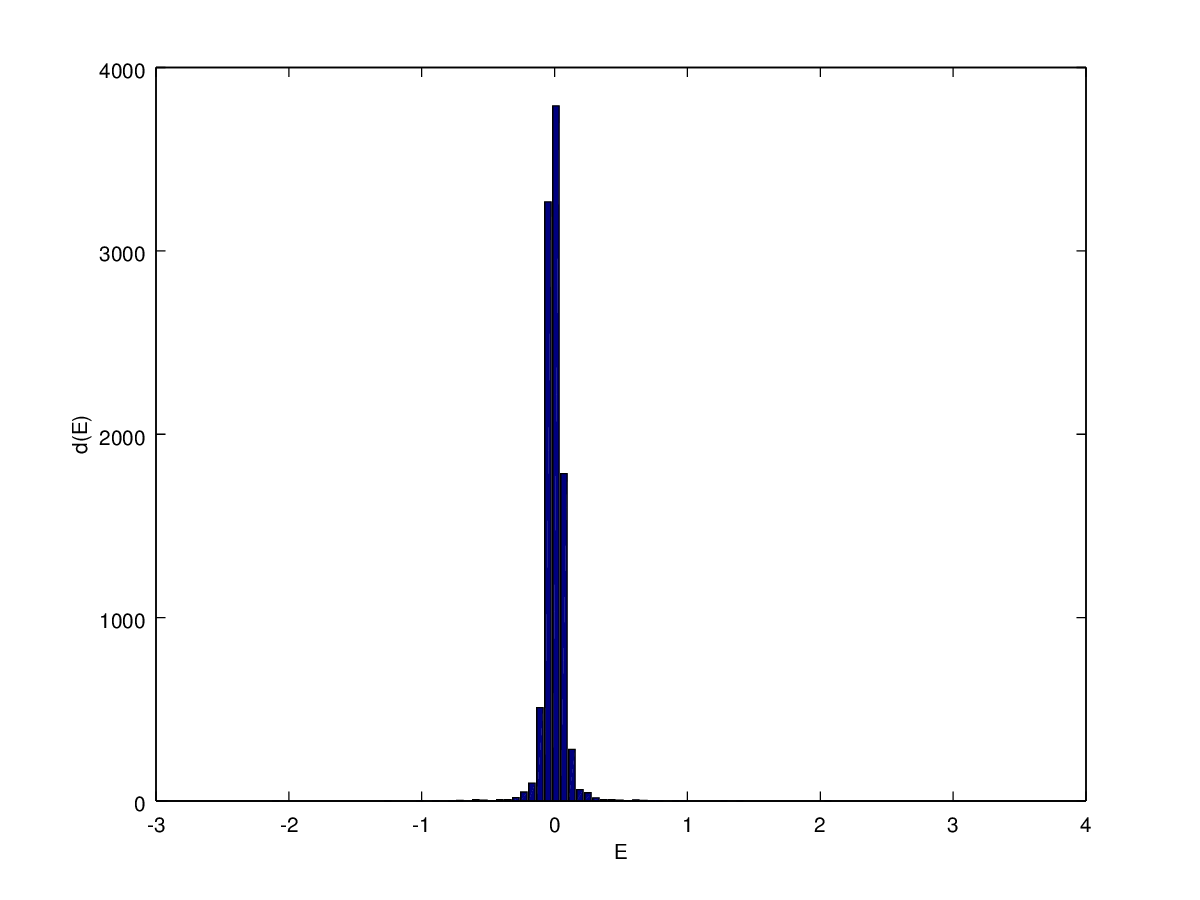
\includegraphics[scale=.50]{veryCloseDos.png}
\caption{The density of states for a system with a high amount of randomness in the energy.}
\label{moundDoS}
\end{center}
\end{figure}

\begin{figure}[htbp]
\begin{center}
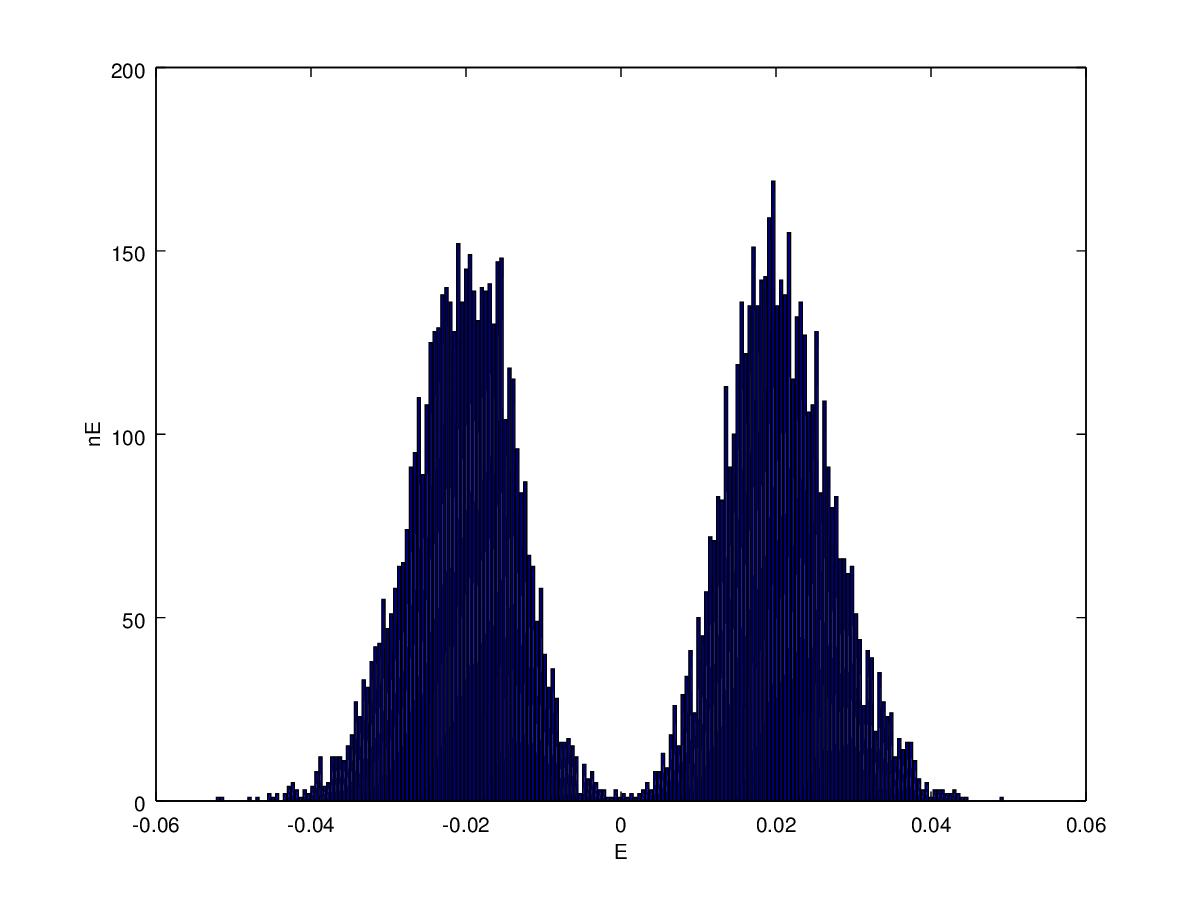
\includegraphics[scale=.50]{critDoS.png}
\caption{The density of states for a system where there is a critical amount of randomization and the two peaks are just beginning to touch.}
\label{critDoS}
\end{center}
\end{figure}


\begin{figure}[htbp]
\begin{center}
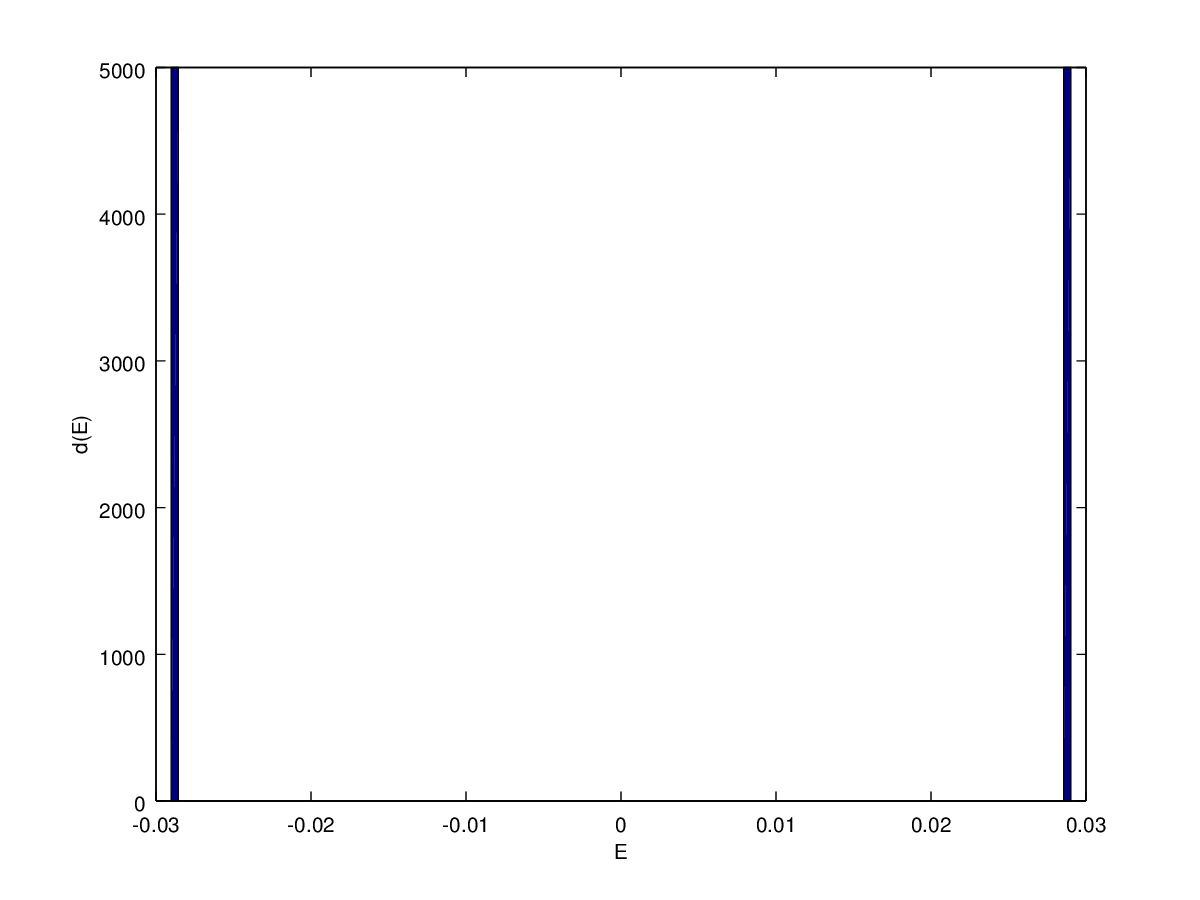
\includegraphics[scale=.50]{splitDos.png}
\caption{A low entropy system (Wigner crystal).}
\label{crystalDoS}
\end{center}
\end{figure}




